\subsection{Introduction}

ResNet-152 solves the vanishing-gradient problem that limits plain very-deep
convolutional networks by learning a residual mapping
$F(x,\{W_i\})$ rather than a direct mapping $H(x)$, and reconstructing the
desired output as $y = F(x,\{W_i\}) + x$ via an identity shortcut. This
section investigates that design empirically along four axes: how well a
frozen, ImageNet-pretrained ResNet-152 transfers to CIFAR-10 as a fixed
feature extractor; what happens to training dynamics and accuracy when
individual identity shortcuts are surgically removed; how class separability
evolves across the network's depth; and how the choice of \emph{which}
layers to fine-tune trades off compute against accuracy. A fifth, optional
set of experiments compares dimensionality-reduction methods, analyzes the
model's confusions directly in feature space, and contrasts ResNet-152
against the shallower ResNet-18 on the same pipeline.

\subsection{Methodology}

\subsubsection{Model, Dataset, and the Frozen-Backbone Pipeline}

All experiments use \texttt{torchvision}'s \texttt{ResNet-152}, pretrained
on ImageNet, applied to CIFAR-10 (10 classes, resized to $224\times224$ and
normalized with ImageNet statistics). Section 1 establishes the baseline
protocol used throughout: every backbone parameter is frozen
(\texttt{requires\_\allowbreak grad\allowbreak=\allowbreak False}) and only a newly-initialized linear
classification head is trained, using a train/validation subset (batch size
$64$) for computational tractability. Because the backbone is frozen and
never updated, its per-image features are identical on every epoch; the
pipeline exploits this by extracting and caching backbone features once
(in \texttt{fp16} to control memory) and training the linear head directly
on the cached features thereafter, avoiding a redundant $152$-layer forward
pass every epoch.

\subsubsection{Residual-Connection Ablation}

To isolate the causal effect of a single identity shortcut, one residual
block's skip connection is disabled in the forward pass -- its output
becomes $y=F(x,\{W_i\})$ instead of $y=F(x,\{W_i\})+x$ -- while every other
block in the $152$-layer network is left untouched. Two qualitatively
different blocks are ablated to test whether \emph{location} matters:
\texttt{layer3[0]}, a \emph{transition} block that also carries a
learned $1{\times}1$ convolutional downsample shortcut (so removing the
identity here removes only the additive skip, not all information flow),
and \texttt{layer3[10]}, an \emph{interior} block with a pure identity
shortcut and $35$ further identity-connected blocks downstream of it within
\texttt{layer3} alone. Both ablated variants are trained and evaluated with
the identical frozen-backbone protocol as the baseline, so any accuracy gap
is attributable to the single removed shortcut.

\subsubsection{Feature Hierarchy Extraction}

Per-image activations are pulled from three depths of the network --
\texttt{conv1} (early, post-stem, before any residual stage),
\texttt{layer3} (middle), and \texttt{avgpool} (late, the $2048$-d
pooled representation Section 1's classifier is trained on) -- via forward
hooks, on a fixed $1000$-image test subset. Each stage's features are
separately projected to 2-D with t-SNE ($\text{perplexity}=30$, PCA
initialization) to visualize how class structure emerges with depth.

\subsubsection{Transfer-Learning Matrix}

Five configurations are trained and compared on identical
data/hyperparameter budgets except where noted: (1) frozen backbone,
pretrained weights, head only (Section 1's baseline); (2) frozen backbone,
\emph{randomly-initialized} weights, head only -- an architecture-only
control; (3) \texttt{layer4} (final residual stage) + head unfrozen,
pretrained weights; (4) \texttt{layer4} + head unfrozen, random-init
weights; (5) the entire backbone unfrozen, pretrained weights, fine-tuned
end-to-end with a reduced learning rate ($10^{-5}$ vs.\ $10^{-4}$ elsewhere)
and fewer epochs ($3$ vs.\ $5$) to avoid destroying the pretrained weights.
Configurations that unfreeze parameters no longer benefit from one-time
feature caching to the same degree, since only the frozen prefix
(\texttt{conv1}--\texttt{layer3} for configs 3--4) can still be cached.

\subsubsection{Optional: Dimensionality Reduction, Confusion Analysis, and ResNet-18}

The late-stage ($\texttt{avgpool}$) features from the $1000$-image subset
are additionally projected with UMAP ($15$ neighbors, $\text{min\_dist}=0.1$)
for comparison against t-SNE. A confusion matrix over the same subset is
paired with pairwise cosine similarity between class centroids in
late-stage feature space, to test whether confused class pairs are also the
pairs with the closest centroids. Finally, the entire frozen-backbone
pipeline (Section 1 protocol) is repeated with \texttt{ResNet-18} in place
of \texttt{ResNet-152}, on the same data split, to compare feature quality
from a much shallower network.

\subsection{Results}

\subsubsection{Baseline}

\begin{figure}[t]
\centering
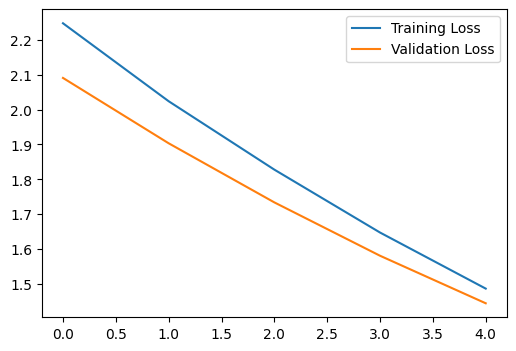
\includegraphics[width=0.9\linewidth]{assets/resnet_fig1.png}
\caption{Baseline training/validation loss, frozen backbone + linear head, 5 epochs.}
\label{fig:resnet-baseline-loss}
\end{figure}

\begin{figure}[t]
\centering
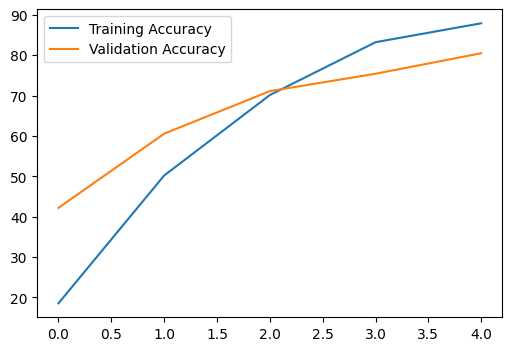
\includegraphics[width=0.9\linewidth]{assets/resnet_fig2.png}
\caption{Baseline training/validation accuracy. Validation accuracy is still rising at epoch 5 (final test accuracy 81.95\%).}
\label{fig:resnet-baseline-acc}
\end{figure}

With only a linear head trained on frozen, ImageNet-pretrained features,
the model reaches $81.95\%$ test accuracy on CIFAR-10 in $5$ epochs
(Figures~\ref{fig:resnet-baseline-loss}--\ref{fig:resnet-baseline-acc}).
Both training and validation accuracy are still climbing at epoch 5 with no
sign of a plateau, indicating the linear probe has not yet converged to its
ceiling under this budget.

\subsubsection{Residual-Connection Ablation}

\begin{figure}[t]
\centering
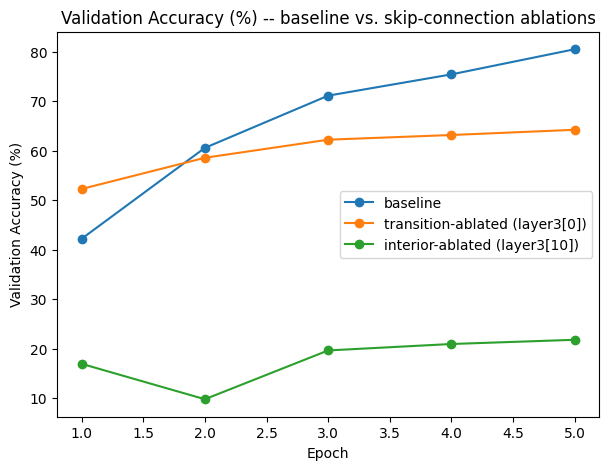
\includegraphics[width=0.9\linewidth]{assets/resnet_fig7.png}
\caption{Validation accuracy: baseline vs.\ transition-block-ablated (\texttt{layer3[0]}) vs.\ interior-block-ablated (\texttt{layer3[10]}).}
\label{fig:resnet-ablation-acc}
\end{figure}

\begin{figure}[t]
\centering
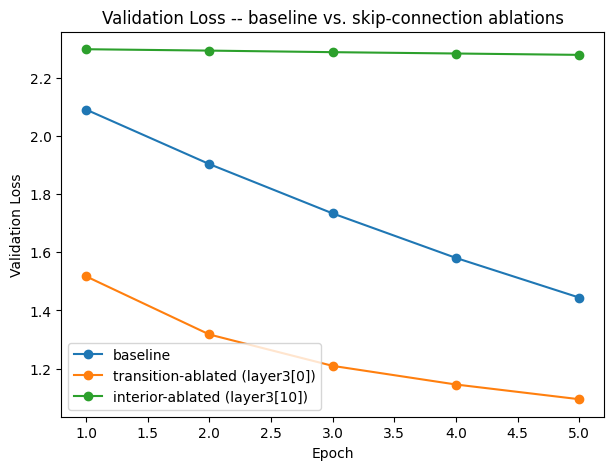
\includegraphics[width=0.9\linewidth]{assets/resnet_fig8.png}
\caption{Validation loss for the same three variants. Note the interior-ablated curve sitting flat near $\ln(10)\approx2.303$ throughout training.}
\label{fig:resnet-ablation-loss}
\end{figure}

Removing the transition block's shortcut (\texttt{layer3[0]}) drops test
accuracy from $81.95\%$ to $64.10\%$; removing the interior block's shortcut
(\texttt{layer3[10]}) drops it to $22.35\%$, barely above the $10\%$ chance
floor. Feature-vector norms at \texttt{avgpool} confirm a mechanistic
difference in severity: the transition ablation leaves the mean norm nearly
unchanged ($15.16\to14.15$, std $2.93\to1.19$), while the interior ablation
collapses it (mean $15.16\to3.38$, std $2.93\to0.31$). Figure~\ref{fig:resnet-ablation-loss}
shows the interior-ablated validation loss sitting essentially flat at
$\approx2.30$ for the entire run -- matching $\ln(10)$, the loss of a
uniform $10$-class distribution, and quantitatively confirming a
degenerate, non-informative regime rather than a merely worse-but-functioning one.

\subsubsection{Feature Hierarchies}

\begin{figure}[t]
\centering
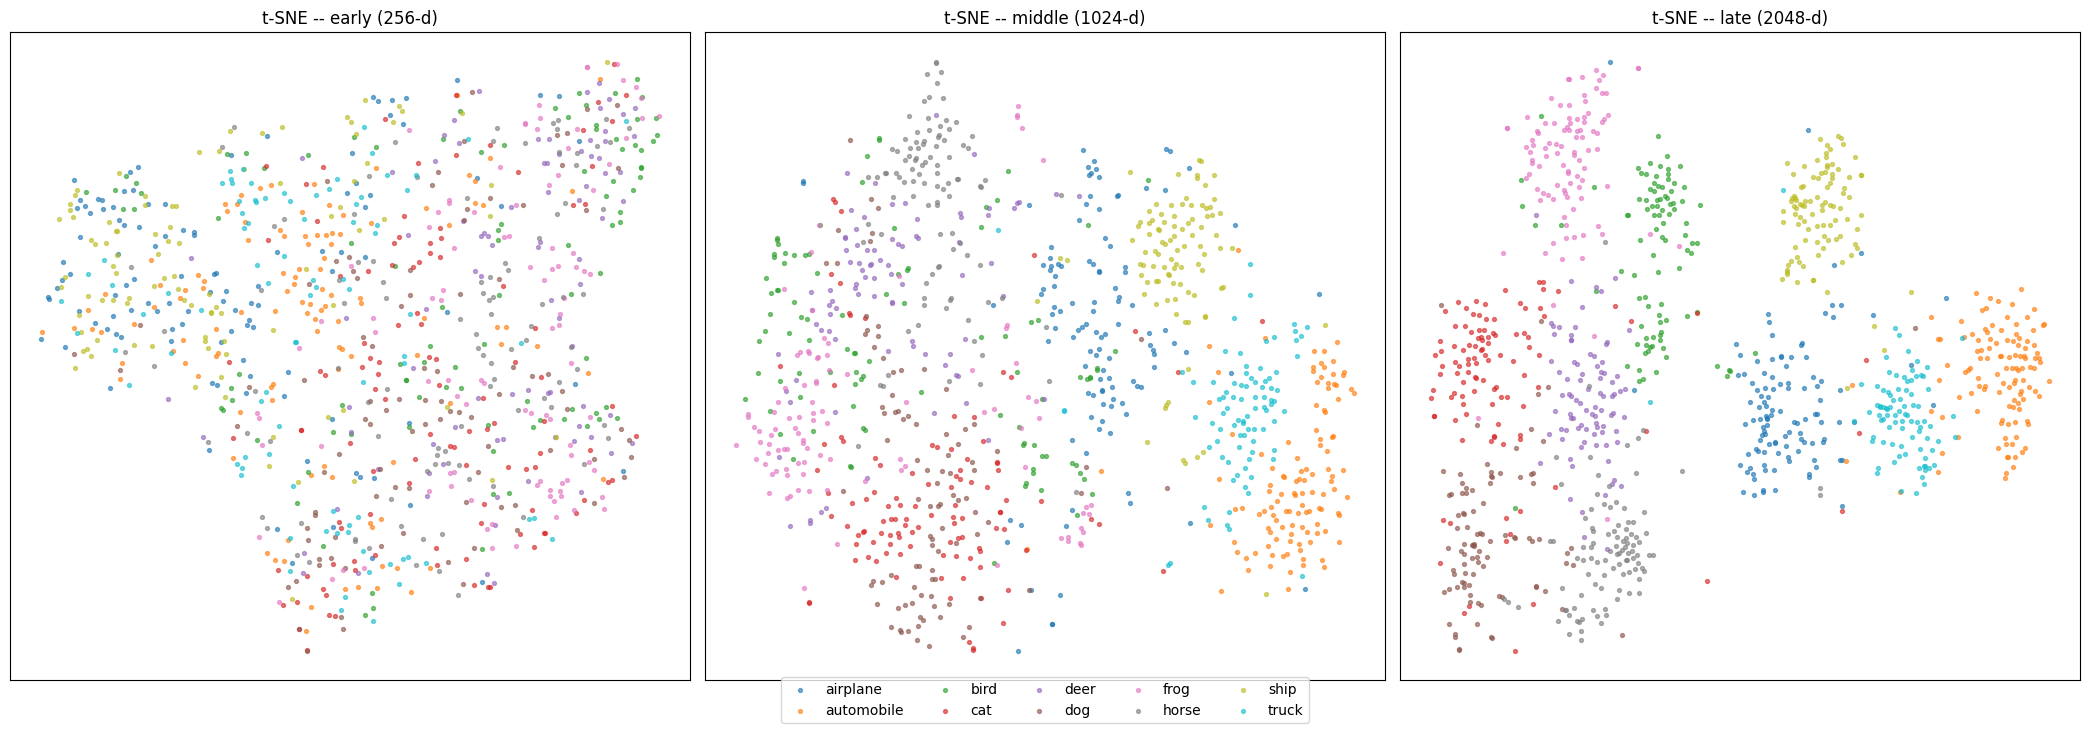
\includegraphics[width=\linewidth]{assets/resnet_fig10.png}
\caption{t-SNE of activations at three depths (1000-image test subset): \texttt{conv1} (early, 256-d), \texttt{layer3} (middle, 1024-d), \texttt{avgpool} (late, 2048-d).}
\label{fig:resnet-tsne-hierarchy}
\end{figure}

Figure~\ref{fig:resnet-tsne-hierarchy} shows a clear progression: early
features show no visible class structure; middle features show partial
separation, with vehicle classes (airplane, automobile, truck) beginning to
separate while several animal classes remain entangled; late features form
ten largely distinct clusters, organized into a coarse vehicle region
(airplane, automobile, truck adjacent to one another) and an animal region
(cat, deer, dog, horse loosely grouped), with bird, frog, and ship forming
their own outlying clusters.

\subsubsection{Transfer-Learning Matrix}

\begin{figure}[t]
\centering
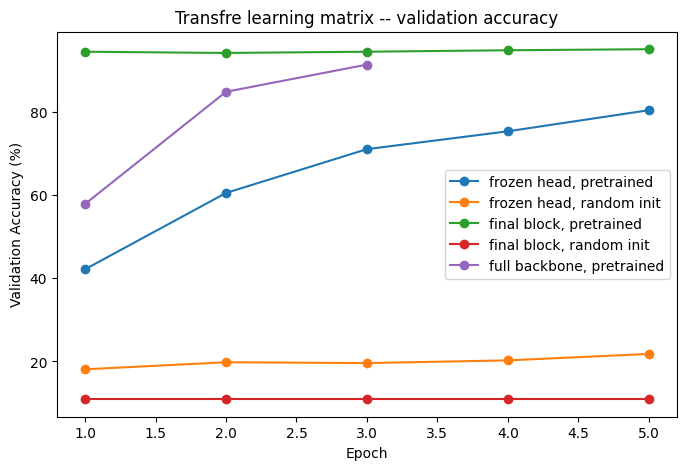
\includegraphics[width=0.9\linewidth]{assets/resnet_fig19.png}
\caption{Validation accuracy across all five transfer-learning configurations.}
\label{fig:resnet-transfer-matrix}
\end{figure}

\begin{table}[t]
\centering
\caption{Final test accuracy, five transfer-learning configurations.}
\label{tab:resnet-transfer}
\begin{tabular}{lcc}
\hline
Setting & Trainable & Test acc.\\
\hline
Final block, pretrained & $\sim$15M & \textbf{94.90\%}\\
Full backbone, pretrained & $\sim$60M & 92.30\%\\
Frozen head, pretrained & $\sim$20K & 81.95\%\\
Final block, random init & $\sim$15M & 11.05\%\\
Frozen head, random init & $\sim$20K & 10.30\%\\
\hline
\end{tabular}
\end{table}

Unfreezing only the final residual stage (\texttt{layer4}) on top of
pretrained weights achieves the best result on both axes simultaneously:
the highest accuracy ($94.90\%$) at a fraction of full fine-tuning's
trainable-parameter cost. Unfreezing the entire pretrained backbone
achieves \emph{lower} accuracy ($92.30\%$) than unfreezing \texttt{layer4}
alone, despite strictly more capacity. Both random-initialization controls
collapse to chance level ($10$--$11\%$), isolating that the gains above come
from the pretrained weights, not the architecture.

\subsubsection{Optional Experiments}

\begin{figure}[t]
\centering
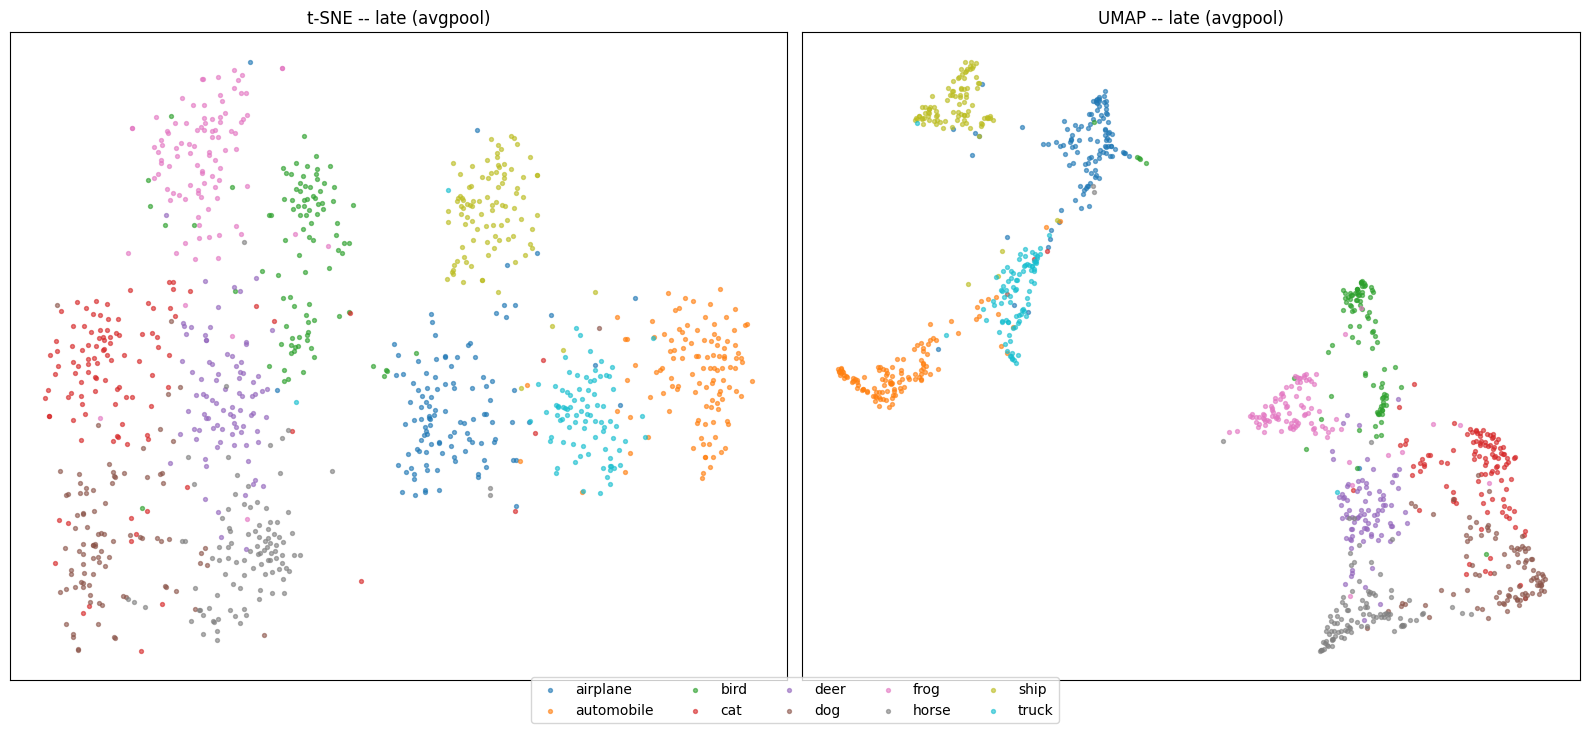
\includegraphics[width=\linewidth]{assets/resnet_fig20.png}
\caption{t-SNE vs.\ UMAP on the same late-stage (\texttt{avgpool}) features, 1000-image subset.}
\label{fig:resnet-tsne-umap}
\end{figure}

\begin{figure}[t]
\centering
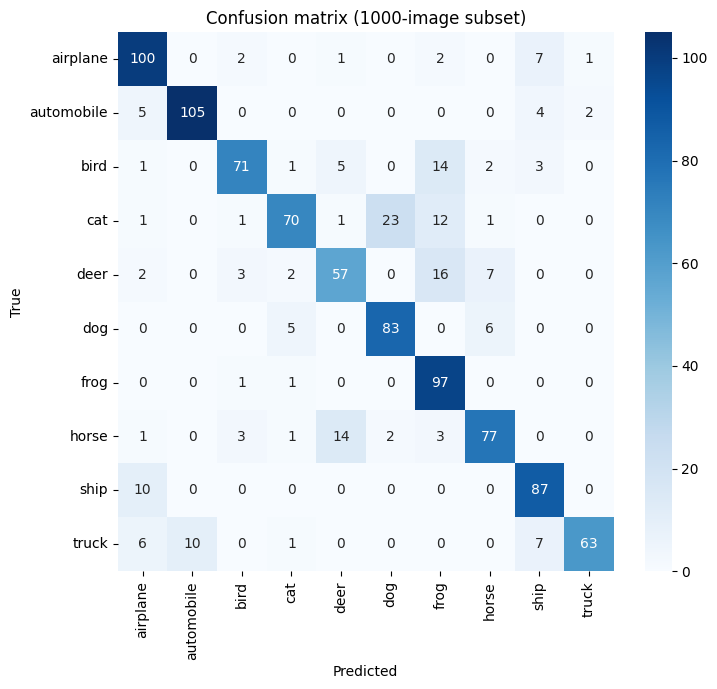
\includegraphics[width=0.85\linewidth]{assets/resnet_fig21.png}
\caption{Confusion matrix, 1000-image test subset, frozen-backbone baseline classifier.}
\label{fig:resnet-confmat}
\end{figure}

\begin{figure}[t]
\centering
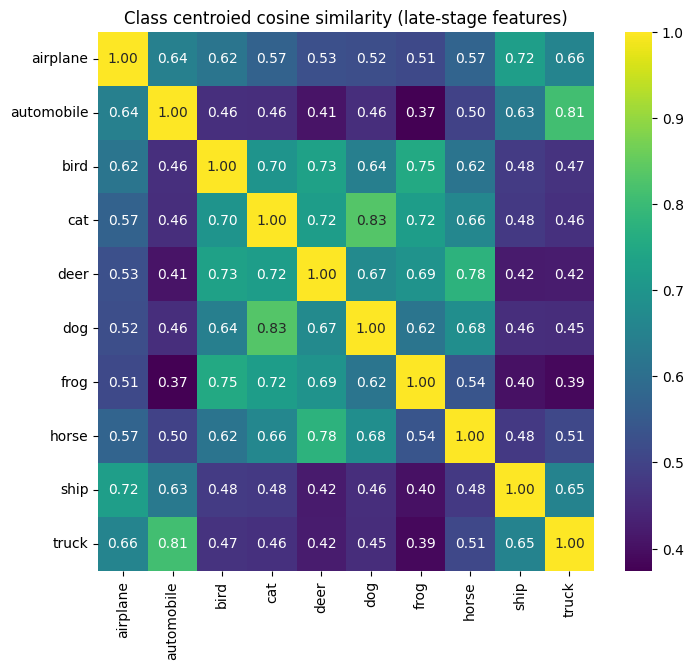
\includegraphics[width=0.85\linewidth]{assets/resnet_fig22.png}
\caption{Cosine similarity between class centroids in late-stage feature space.}
\label{fig:resnet-centroid-sim}
\end{figure}

\begin{figure}[t]
\centering
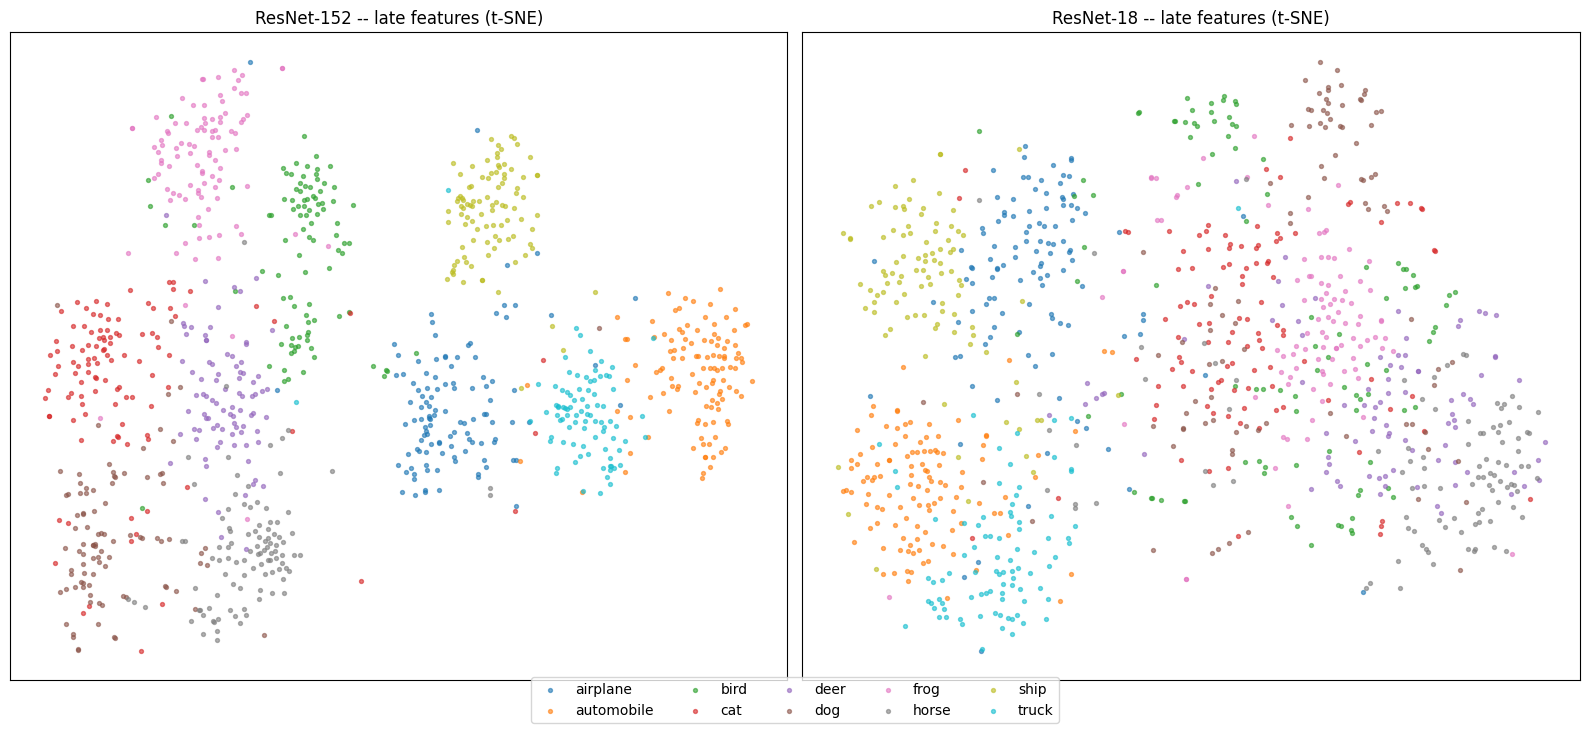
\includegraphics[width=\linewidth]{assets/resnet_fig25.png}
\caption{t-SNE of late-stage features, ResNet-152 (left) vs.\ ResNet-18 (right), same 1000 test images.}
\label{fig:resnet18-vs-152-tsne}
\end{figure}

UMAP (Figure~\ref{fig:resnet-tsne-umap}, right) preserves the same
vehicle/animal grouping as t-SNE but renders it as a more continuous,
connected trail between related classes (ship--truck--automobile) rather
than t-SNE's more discrete islands. The confusion matrix
(Figure~\ref{fig:resnet-confmat}) shows the largest off-diagonal
confusions are cat$\to$dog ($23$ of $206$ predictions),
deer$\leftrightarrow$horse ($16$/$14$), bird$\to$frog ($14$), and
automobile$\leftrightarrow$truck ($10$/$7$). These are exactly the pairs
with the highest centroid cosine similarity in
Figure~\ref{fig:resnet-centroid-sim}: cat--dog $0.83$, deer--horse $0.78$,
automobile--truck $0.81$ -- each the single highest off-diagonal value in
its respective row.

Repeating the frozen-backbone pipeline with ResNet-18 (11{,}181{,}642
parameters vs.\ ResNet-152's 58{,}164{,}298) gives a \emph{higher} test
accuracy of $84.30\%$, versus ResNet-152's $81.95\%$. However,
Figure~\ref{fig:resnet18-vs-152-tsne} shows the opposite pattern in feature
space: ResNet-152's late features form visibly cleaner, more separated
clusters, while ResNet-18's are substantially more entangled and overlapping
for the same $1000$ images.

\subsection{Discussion}

\subsubsection{Why Frozen-Feature Transfer Works, and Why Training From Scratch Is Not Viable Here}

ResNet-152 has $58{,}164{,}298$ parameters against a CIFAR-10 training
subset of $8{,}000$ images -- a parameter-to-example ratio of roughly
$7{,}270{:}1$. Optimizing a model this overparameterized from random
initialization on this little labeled data is severely underdetermined:
with thousands of free parameters per training image, gradient descent has
enormous freedom to fit idiosyncrasies of those specific $8{,}000$ images
rather than being forced to discover generalizing structure, on top of
needing far more compute than the task justifies for a $152$-layer network.
It would also have to rediscover the entire feature hierarchy -- edges,
textures, parts, object shape -- from scratch using only those examples,
with nothing priming it toward image-general structure the way ImageNet
pretraining does.

Freezing the backbone entirely and training only a linear head
(Section~1) is a controlled experiment for exactly this question: are the
frozen, never-CIFAR-10-touched ImageNet features already close to linearly
separable for $10$ classes the network was never explicitly trained to
distinguish? Reaching $81.95\%$ test accuracy from a linear read-out alone
says yes. This is corroborated, not merely asserted, by the random-init
control in Section~4: repeating the identical frozen-head protocol with a
randomly-initialized backbone collapses accuracy to $10.30\%$, chance
level for $10$ classes. Since the only difference between that run and the
$81.95\%$ baseline is the \emph{origin} of the frozen weights, the entire
gap is attributable to the transferability of the pretrained representation
itself, not to having a $152$-layer architecture available -- direct
evidence that the transferable knowledge lives in the representation, not
in the classifier trained on top of it.

\subsubsection{Why the Identity Shortcut Matters, and Why Location Changes the Severity}

Backpropagating through $y=F(x,\{W_i\})+x$ gives
$\partial L/\partial x = (\partial L/\partial y)(\partial F/\partial x + I)$:
the additive identity guarantees a direct gradient path back to $x$
regardless of how small $\partial F/\partial x$ becomes. Removing it leaves
only $\partial y/\partial x = \partial F/\partial x$, so if $F$'s Jacobian
has small singular values -- plausible in a $152$-layer pretrained network
whose blocks were never trained without their shortcuts -- the signal
through that point becomes unreliable. This alone would predict some
degradation at either ablated block, but not the roughly $3\times$
larger accuracy drop observed at the interior block versus the transition
block. The transition block (\texttt{layer3[0]}) still has a learned
$1{\times}1$ projection carrying information forward even without the
additive identity, and the $35$ subsequent interior blocks in
\texttt{layer3} retain their own intact shortcuts, giving the network many
remaining chances to partially compensate. The interior block
(\texttt{layer3[10]}) has no such fallback: its removal desynchronizes the
running residual sum from what every one of the $25$ \emph{subsequent}
interior blocks' BatchNorm statistics were calibrated against during
ImageNet pretraining, and that mismatch compounds rather than being
absorbed -- consistent with the feature-norm collapse (std $2.93\to0.31$)
and the loss curve sitting at the uniform-distribution floor.

A subtlety in Figure~\ref{fig:resnet-ablation-loss} is worth flagging: the
transition-ablated model's validation \emph{loss} is lower than the
baseline's throughout training, despite scoring $18$ points lower on
accuracy. Cross-entropy loss and accuracy are not the same objective --
this model's degraded, lower-variance features produce a more collapsed
output distribution that happens to minimize average cross-entropy more
easily without being more discriminative, which is exactly why loss alone
is an unreliable proxy for classification quality when the underlying
representation has been damaged.

\subsubsection{Why Class Structure Emerges Only at Depth}

\texttt{conv1}'s receptive field is small, so its channels respond to
local texture/edge statistics -- information necessary for recognizing an
object but not sufficient on its own, since class identity is a global,
compositional property. Euclidean distance in that space mostly reflects
texture similarity, not semantic similarity, which is why same-class images
do not cluster there. By \texttt{avgpool}, the receptive field spans the
full input after four residual stages of downsampling and composition, and
the network was specifically optimized (via ImageNet pretraining) to make
class-discriminative decisions from exactly this representation --
$81.95\%$ test accuracy from a \emph{linear} probe on these features
(Section 1) is the quantitative confirmation of what
Figure~\ref{fig:resnet-tsne-hierarchy} shows qualitatively. The
vehicle/animal grouping visible at the late stage is a coarser semantic
hierarchy inherited from ImageNet's broader $1000$-class structure, above
and beyond the $10$-way distinction CIFAR-10 actually asks for.

\subsubsection{Compute/Accuracy Trade-off and Layer Transferability}

Unfreezing only \texttt{layer4} wins on both axes because it matches the
standard dataset-size $\times$ domain-similarity heuristic for transfer
learning: CIFAR-10 is small ($8000$ training images) and domain-similar to
ImageNet (both natural photographs), which calls for adapting only the
final, most task-specific layers rather than fine-tuning everything. Full
backbone fine-tuning has roughly $4\times$ more trainable parameters than
an $8000$-image budget can reliably constrain, and required a smaller
learning rate and fewer epochs specifically to avoid destroying the
pretrained weights -- and it still underperforms \texttt{layer4}-only
fine-tuning. This is direct evidence that \texttt{conv1}--\texttt{layer3}
are already close to optimally transferable for this target domain, and
adapting them under this data budget does more harm (mild overfitting)
than good; \texttt{layer4} is where the useful task-specific adaptation
actually happens. The random-init controls isolate that every benefit
above comes from the ImageNet-pretrained weights, not from having a
$152$-layer architecture available.

\subsubsection{Confusions Are Predictable from Feature-Space Geometry}

The confusion matrix and centroid-similarity heatmap tell the same story
from two different angles: every class pair with a large off-diagonal
confusion count is also the pair with the highest centroid cosine
similarity in that row. This is consistent with a linear classifier
operating on these features -- decision boundaries between classes whose
centroids sit close together in $2048$-d space are inherently thinner
margins, so any given test point is more likely to fall on the wrong side.
It also explains \emph{which} confusions occur along semantic lines
(cat/dog, deer/horse, automobile/truck) rather than arbitrarily: these are
exactly the categories that share the most visual attributes (fur texture
and body shape for the animal pairs; wheeled, boxy silhouettes for the
vehicle pair), and the frozen ImageNet backbone encodes that visual
similarity directly into feature-space proximity.

\subsubsection{Accuracy and Representation Quality Are Not the Same Thing}

The ResNet-18 comparison is the most counter-intuitive result in this
section: ResNet-18 achieves \emph{higher} test accuracy ($84.30\%$ vs.\
$81.95\%$) with roughly $5\times$ fewer parameters, yet its late-stage
features are visibly \emph{less} well-separated by unsupervised
visualization (Figure~\ref{fig:resnet18-vs-152-tsne}) than ResNet-152's.
The resolution is that these are different measurements: test accuracy
reflects what a fully-trained \emph{linear classifier} can extract from the
features, using all $512$ (ResNet-18) or $2048$ (ResNet-152) dimensions and
a supervised decision boundary optimized specifically for this task, while
t-SNE is an unsupervised, 2-D, distance-preserving projection that discards
information a linear classifier can still use. A representation can be
messier to look at in two dimensions while still being more linearly
separable in its native, much higher-dimensional space -- ResNet-18's
smaller capacity and different pretraining trajectory may in fact yield
features that are more \emph{efficiently} discriminative for this specific
10-class problem, even though they are not visually as cleanly clustered.
This is a useful caution against reading representation quality off a
single 2-D visualization alone.
